   
%! Tree and Queues
%! Author = Vincent Ferrigan <ferrigan@kth.se>
%! Date = 2022-10-07


% Preamble
\documentclass[a4paper, 11pt]{article}
% Packages
\usepackage[T1]{fontenc}
\usepackage[utf8]{inputenc}
\usepackage[english]{babel}
\usepackage{fontspec}
\usepackage{polyglossia}
\usepackage{microtype}
\setmonofont{DejaVu Sans Mono}[Scale=MatchLowercase]
\usepackage{listings}
\usepackage{minted}
\usepackage{latexsym,exscale,stmaryrd,amsmath,amssymb}
\newtheorem{definition}{Definition}
\usepackage{unicode-math}
\usepackage{lmodern}
\usepackage{enumitem}
\usepackage{subcaption}
\usepackage{graphicx}
\usepackage{hyperref}
\usepackage{multirow}
% \usepackage{paralist}

%% Om jag vill referera till ett kod verb av något slag, som void null Int etc
% \usepackage{tcolorbox}
% \newtcbox{\somestuffstyle}{on line,boxrule=0pt,boxsep=0pt,colback=lightgray,top=1pt,bottom=1pt,left=1pt,right=1pt,arc=0pt,fontupper=\ttfamily}

% \usepackage{natbib}
% \usepackage[nottoc]{tocbibind}
\usepackage{xcolor}
\usepackage{siunitx}
\usepackage{tikz}
\usepackage[font=small,labelfont=bf]{caption}
% Addiding JuliaMono
\newfontfamily \JuliaMono {JuliaMono-Regular.ttf}[
    Path      = ./,
    Extension = .ttf
    ]
\newfontface \JuliaMonoMedium{JuliaMono-Regular}
\setmonofont{JuliaMonoMedium}[
    Contextuals=Alternate
]

\title{Trees on stacks and queues\\ \small{ID1021 Algorithms and Data structures}} %%TODO vilken rubricering
\author{Vincent Ferrigan}

\date{\today}

\begin{document}
    \maketitle
    \section*{Introduction}
    \label{sec:introduction}
    In this paper, the performance and implementation of two data structures, 
    the \emph{binary search tree} and the \emph{queue} were studied and analyzed. 
    Several tree algorithms were also studied. 
    A \emph{lookup algorithm} was compared with the binary search algorithm 
    (studied in a previous paper).  % ska jag lägga till ref?
    This was done through benchmarking -- i.e. comparing the performance of
    the two data algorithms in terms of managing data. E.g. how well do these
    algorithms' scale with the size of the input data? 
    Does the shape of the tree matter during lookup? That is, when 
    constructing a tree, does the order of adding nodes matter? 
    Essentially affecting both the shape of the tree and its height. % mer en konklution 

    The final task was to implement iterators for traversing a binary tree 
    based on two approaches 
    -- \emph{Depth First} and \emph{Breadth First}. 
    Which were implemented using \emph{stacks} and \emph{queues}.
    The question is, in what order do we apply Depth First? 
    \emph{In-order}, \emph{pre-order} or \emph{post-order}? 
    All four \emph{Traversal Algorithms} where studied. 
    
    The authors intent is to reach certain conclusions on the queries that were
    stated above. 
    
    \section*{Methods}
    All the Data Structures and Algorithms were implemented in \emph{Julia}.
    The Code was mostly written in \emph{VSCode} and run on \emph{Julia 1.8.0}.
    Quick-fixes and editing was, however, done in \emph{Vim}

    Some scripts were executed from the \emph{REPL terminal},  while others (e.g.
    when using data frames, performing benchmarks and producing plots) 
    were executed from the \emph{Jupyter Notebook}. 
    % Ska jag lägga till länk till min github? To follow the progress.....
    % men då måste notebooken läggas upp.
    
    \subsection*{Tools and packages}
    All tests were performed with the built-in package \emph{Test} and 
    iterative development was made possible through 
    \emph{Revise.jl} -- the latter operates by continuously
    scanning the source code for changes, even changes in functions defined in
    other modules (including modules written in different files).
    
    The benchmark data was constructed, manipulated and visualized through
    \emph{DataFrames.jl} and \emph{Plots.jl}, 
    while readable formatting was produced through 
    \emph{Formatting.jl} and \emph{Unitful.jl}. 

    \subsection*{The JIT}
    Julia has a just-in-time (JIT) compilation -- which means that the code is
    dynamically compiled during program run time.     
    It takes time for the JIT compiler to 
    initially load the code and compile it. Therefore, in order not to skew the
    results, \emph{warm-up calls} were performed on certain parts of the code
    before they were benchmarked. This to avoid including 
    compilation time. The warm-up calls were done with the @timed macro prior to
    benchmarking.

    \section*{The Data Structure}
    This section briefly describes the key differences between \emph{binary trees} 
    and other data structures -- such as \emph{linked lists} and \emph{vectors}. 
    It will also illustrate how both \emph{stacks} and \emph{queues} were used
    when implementing \emph{traversal algorithms}. 
    The implementation of both the lookup and traversal algorithms will also be
    depicted by this section.
    
    For clarity, the reader is given meaning to the terms dealing 
    with binary trees -- not only with descriptions of the
    ''tree-terms'' used in this paper, but also with a specification 
    of the overall implementation in Julia. The reader will also be provided with 
    code examples when necessary.

    \subsection*{Conventions}
    It is important for the reader to note that Julia uses a one-based-numbering
    convention, (i.e. array indices start from 1 to N) and that one dimensional
    arrays are called vectors. 
    For consistency, the author has chosen to refer to one dimensional
    arrays as vectors and apply the 1-based convention when numbering
    sequences of elements more broadly. 
    
    Unlike other languages, Julia objects cannot be ''null'' by default. The
    equivalent of \lstinline[language=Python]{None} in Python or
    \lstinline[language=C]{NULL} and \lstinline[language=C]{void} in C is
    \mintinline{julia}{Nothing}. The Julia convention is to return the value
    \mintinline{julia}{nothing}, which is a singleton instance of type
    \mintinline{julia}{Nothing}, when such a side effect is
    desired. 

    \clearpage
    \subsection*{The Binary Tree}
    \label{sec:thebinarytree}
    Like \emph{linked lists}, \emph{binary trees} are dynamic data structures that, unlike \emph{vectors}, 
    do not require to be stored contiguously in memory. They are instead composed of \emph{nodes} 
    that are linked together by pointers or references. 
    Like the implementation of linked lists, the tree requires two data structures; one
    for the actual node and another for the tree, the latter containing a
    reference that points to the first node. 
    Each node in the binary tree that was implemented in this paper, contains five parts;
    % \begin{inparaenum}[i)]
    \begin{enumerate}[itemsep=1pt]
        \item a \mintinline{julia}{key} of any type \mintinline{julia}{K}
        \item a \mintinline{julia}{value} of any type \mintinline{julia}{V} 
        that is associated with the key
        \item a reference (memory address) to the linked node \mintinline{julia}{left}
        \item a reference (memory address) to the linked node \mintinline{julia}{right} and
        \item the number of nodes \mintinline{julia}{n} in the tree/subtree. 
        A number that that includes the node itself as well as all its descendants.
    \end{enumerate}
    % \end{inparaenum}

    The fields that contain references to other nodes may point to nothing 
    which, as previously mentioned, is a singleton instance of type \mintinline{julia}{Nothing}.
    \autoref{code:node} shows how the above-mentioned nodes were implemented in Julia. 
    Since the fields \mintinline{julia}{left} and \mintinline{julia}{right} only sometimes 
    contain a reference to another node, the data type \mintinline{julia}{Union} was used for their 
    field declaration -- a union that includes the composite
    data type (for the node in question) and `nothing`.

    The first node in the tree is conventionally called \emph{the root}, as in the root of the tree.
    The tree therefore usually only contains one item, the reference to the first node, the root that is.
    See \autoref{code:binarytree}. Apart from the root, 
    each node in a binary tree is pointed to by just one other node, which is called its \emph{parent}. 
    At most, every node can have two children, the first is called the \emph{left child}
    and the second is called the \emph{right child}.  
    \begin{figure}[h]
        \centering
    \begin{minted}[
        label= Node Data Type (Custom Struct),
        linenos, 
        % breaklines, 
        frame = single, 
        fontsize=\footnotesize]{julia}
mutable struct BTNode{K, V} <:MyAbstractTreeNode{K, V} 
    key::K
    value::V
    left::Union{BTNode{K, V}, Nothing}
    right::Union{BTNode{K, V}, Nothing}
    n::Int64 
end
    \end{minted}
    \caption{Node example for Binary Search Trees in Julia}
    \label{code:node}
    \end{figure}

    \clearpage
    A node of a tree is called a \emph{leaf} if it has no children. Nodes that
    have at least one child are called \emph{internal nodes}. 
    The root is internal node unless it is the only node in the tree, in which case it is a leaf. 
    The field \mintinline{julia}{root} in the binary tree (as shown in the
    example in \autoref{code:binarytree})
    can sometimes contain a reference to nothing, in which case the tree is empty.
    The tree rooted at the left child
    of a node is called the \emph{left subtree} of this node, and the tree rooted at the
    right child of the node is called the \emph{right subtree} of the node.
    Since each subtree are themselves binary trees. Two nodes with the same 
    parent are called \emph{siblings}. In this study, the nodes holds neither reference to its parent 
    nor to its sibling -- which affects the traversal of the tree 
    (see subsection \hyperref[sec:treetraversal]{Tree Traversal}).

    The binary tree in this paper is ordered as a \emph{Binary Search Tree (BST)}, that is, 
    the key of a node must be unique and larger than the keys of all nodes in
    its left subtree and smaller than the keys of all the nodes in its right
    subtree. The siblings are therefore ordered from left to right.

    \begin{figure}[h]
        \centering
    \begin{minted}[
        label=Binary Tree Data Type (Custom Struct), 
        linenos, 
        % breaklines, 
        frame = single, 
        fontsize=\footnotesize]{julia}
mutable struct BTree{K, V} <: MyBinaryTree{K, V}
    root::Union{Nothing, BTNode{K, V}}
end
    \end{minted}
    \begin{minted}[
        label=Outer construct, 
        linenos, 
        % breaklines, 
        frame = single, 
        fontsize=\footnotesize]{julia}
BTree{K, V}() where {K, V} = BTree{K, V}(nothing)
    \end{minted}
    \caption{A Binary Search Tree implementation in Julia.}
    \label{code:binarytree}
    \end{figure}

    \clearpage
    \subsubsection*{Adding and updating}
    \label{sec:adding}
    The procedure for adding a new item (consisting of a key and its associated value)
    to the BST requires comparing keys of
    nodes that already exist in the BST. Starting at the root and moving left
    if the new item's key is smaller than visited node or move right if it is larger. 
    The function written for this procedure, as shown in 
    \autoref{code:add!}, adds a new node (leaf) that maps
    given key to value. If the given key is already present, the value that is
    mapped to it gets updated with given value. Essentially turning this function into
    one that not only adds but also updates keys. 
    The add-function is recursive in nature and is therefore implemented with 
    two methods % ska jag lägga till varför det heter metoder i Julia????
    depending on the data type it receives, 
    that is if the data type is a tree or a node. 
    This feature in Julia is known as \emph{multiple dispatch}, 
    which is similar but not equal to \emph{function overloading} in Java and C++. 
    The function name ends with a bang (!) since it mutates the arguments it receives. 
    This name suffix is by convention in Julia. 
    \begin{figure}[H]
        \centering
    \begin{minted}[
        label=Outer method, 
        linenos, 
        % breaklines, 
        frame = single, 
        fontsize=\footnotesize]{julia}
function add!(tree::BTree{K, V}, key::K, value::V) where {K,V}
    tree.root = add!(tree.root, key, value)
    tree
end
    \end{minted}
    \begin{minted}[
        label=Inner method, 
        linenos, 
        % breaklines, 
        frame = single, 
        fontsize=\footnotesize]{julia}
function add!(
    node::Union{BTNode{K, V}, Nothing}, 
    key::K, 
    value::V
    ) where {K,V}
    if isa(node, Nothing)  
        node = BTNode{K, V}(key, value, nothing, nothing, 1)
        return node
    end

    if key < node.key
        node.left = add!(node.left, key, value)
    elseif key > node.key
        node.right= add!(node.right, key, value)
    else
        node.value = value
    end

    node.n = size(node.left) + size(node.right) + 1
    return node
end
    \end{minted}
    \caption{The add or update function 'add!' in Julia.}
    \label{code:add!}
    \end{figure}

    \subsubsection*{Accessing through lookup}
    \label{sec:lookup}
    The procedure of locating an item acts similarly to adding one to
    a BST. 
    The function, which also consist of two methods, is named 'lookup' (in
    accordance with the assigned task) and its Julia code is shown in figure
    \autoref{code:lookup}. The function locates and returns the value associated
    to given key. The methods return 'nothing' if the given key is not found. 
    
    As mentioned in the \hyperref[sec:introduction]{introduction}, 
    it is this function that was benchmarked to 
    a binary search algorithm (see \hyperref[sec:results]{Section Results})

    \begin{figure}[H]
        \centering
    \begin{minted}[
        label=Outer method, 
        linenos, 
        % breaklines, 
        frame = single, 
        fontsize=\footnotesize]{julia}
function lookup(tree::BTree{K,V}, key::K) where {K,V} 
    lookup(tree.root, key)
end
    \end{minted}
    \begin{minted}[
        label=Inner method, 
        linenos, 
        % breaklines, 
        frame = single, 
        fontsize=\footnotesize]{julia}
function lookup(
    node::Union{BTNode{K, V}, Nothing}, 
    key::K
    ) where {K,V}
    
    isa(node, Nothing) && return nothing
    if key < node.key
        lookup(node.left, key)
    elseif key > node.key
        lookup(node.right, key)
    else
        return node.value
    end
end
    \end{minted}
    \caption{The locate function 'lookup' in Julia}
    \label{code:lookup}
    \end{figure}
    In algorithm textbooks one can find other names for the functions described above 
    e.g. the \mintinline{julia}{add!} function is called \emph{'put'} while 
    \mintinline{julia}{lookup} is called \emph{'get'}.
    % ska jag lägga till ref (sedgewick), och även nämna 'search' från Cormen??  


    \subsection*{The Traversal Algorithms}
    \label{sec:treetraversal}
    
    A tree traversal refers to the process of visiting each node in a tree at least once. 
    This ''visit'' can inquire some kind of action, 
    e.g. accessing each node for printing their keys and their associated values. 
    The question of order is of same importance as visiting each node only once. 
    
    \subsubsection*{Downwards or sideways?}
    \label{sec:breadthfirsttraversal}
    The \emph{Depth-First} approach traverses downwards through each branch of a (sub)tree
    before backtracking. It is implemented using a \emph{stack}, which will enable 
    the use of recursion -- since each subtree are themselves binary trees. Compare
    this to the \emph{Breadth-Frist} approach which visits each node sideways,
    level-by-level, requiring a \emph{queue} for its implementation.
    
    There are a few different orders within the Depth First approach. 
    The three that were used in the study are 
    \emph{pre-order}, \emph{in-order} and \emph{post-order}. 

    The development of these traversal algorithms were done 
    through iterative testing. 

    At first, a balanced BST was created by adding key-value pairs in the following 
    order: 
    \begin{minted}[
        % label=codeexample, 
        % linenos, 
        % breaklines, 
        % frame = single, 
        fontsize=\footnotesize]{julia}
tree = BTree{Int64, String}()

add!(tree, 4, "1st")  # Tree      Root    ROOT
add!(tree, 2, "2nd")  # L-Subtree Root    INTERNAL NODE
add!(tree, 1, "3rd")  # L-Subtree L-child LEAF
add!(tree, 3, "4th")  # L-Subtree R-child LEAF
add!(tree, 6, "5th")  # R-Subtree Root    INTERNAL NODE
add!(tree, 5, "7th")  # R-Subtree L-child LEAF
add!(tree, 7, "8th")  # R-Subtree R-child LEAF
    \end{minted}
    
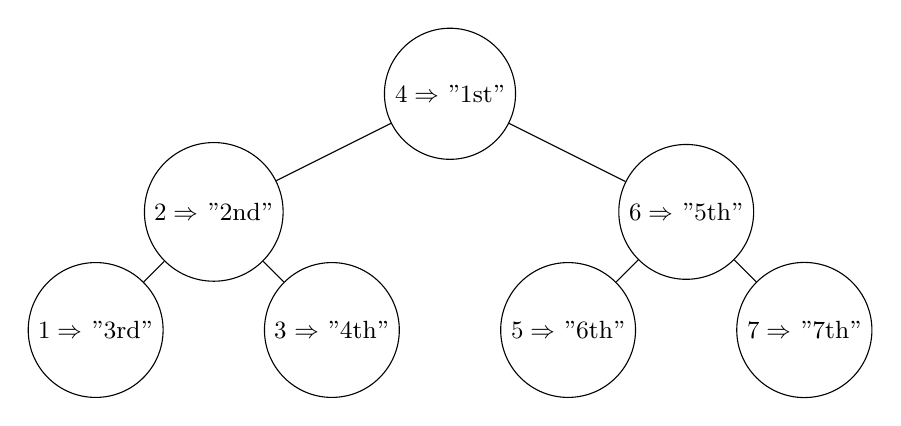
\begin{tikzpicture}[
  every node/.style = {minimum width = 1em, draw, circle},
  level/.style = {sibling distance = 60mm/#1}
  ]
  \small
  \node {$4 \Rightarrow$ "1st"}
  child {node {$2 \Rightarrow$ "2nd"} 
        child {node {$1 \Rightarrow$ "3rd"}}
        child {node {$3 \Rightarrow$ "4th"}}
        }
  child {node {$6 \Rightarrow$ "5th"}
        child {node {$5 \Rightarrow$ "6th"}}
        child {node {$7 \Rightarrow$ "7th"}}
        };
\end{tikzpicture}

    Single line comments in Julia start with the hashtag symbol(\#) and lasts
    till the end of the line. 
    The comments above point to where the nodes are located in the tree. 

    Depending on traversal algorithm, the values were updated and traversed in accordance 
    with \autoref{tab:traversalalgorithms}.
    A \emph{In-order traversal} visits the nodes in key ascending order while the
    \emph{post-order traversal} can be used as a procedure for 
    expression evaluation of Reversed Polish Notation (RPN) -- also called
    postfix notation. RPN is used to express mathematical formulas 
    that do not need the use of 
    brackets to keep the order of precedence. 
    The example found in \autoref{tab:traversalalgorithms} holds the postfix
    expression \mintinline{postscript}{1 2 + 3 4 + *}.

    The print-results were performed with for-loops based on 
    different custom iterators. 
    The formatting was done through \emph{pretty printing}, by overloading the base function show.
    \begin{minted}[
        label=pretty-printing, 
        linenos, 
        % breaklines, 
        frame = single, 
        fontsize=\footnotesize]{julia}
function show(io::IO, node::BTNode{K,V}) where {K,V}
    print(" key: ", node.key, " => value: ", node.value)
end
    \end{minted}
    This paper will focus on two custom iterators. 
    One based on the Pre-order (depth first) approach
    and the other on the breadth-first. 
    The former was implemented using a \emph{stack} while the latter
    used a \emph{queue}

    \subsubsection*{Pre-order traversal}
    A pre-order traversal is used to create copies of binary trees. 
    % A Preorder traversal produces a representation that is the same as the way
    % % that the programming language Lisp processes arithmetic expressions. (PREFIX)
    It also produces a prefix representation of an arithmetic expression. 
    E.g. a program written in a lisp dialect, would write the previously 
    mentioned postfix notation \mintinline{postscript}{1 2 + 3 4 + *} in preorder
    as \mintinline{scheme}{(* (+ 1 2)(+ 3 4))}. 
    This arithmetic expression can also be written with a lisp-like syntax in
    Julia as \mintinline{julia}{*(+(1, 2), +(3, 4))}.

\begin{figure}[h]
\centering
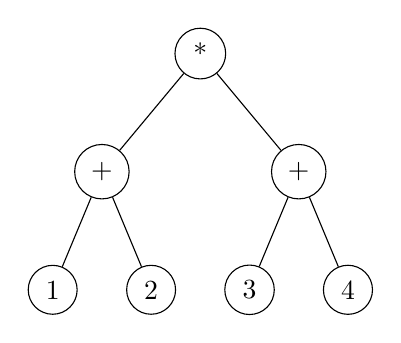
\begin{tikzpicture}[
  every node/.style = {minimum width = 1em, draw, circle},
  level/.style = {sibling distance = 25mm/#1}
  ]
  \node {*}
  child {node {+} 
        child {node {1}}
        child {node {2}}
        }
  child {node {+}
        child {node {3}}
        child {node {4}}
        };
\end{tikzpicture}
\end{figure}
Describe ....
    \begin{figure}[H]
        \centering
    \begin{minted}[
        label=Outer method, 
        linenos, 
        % breaklines, 
        frame = single, 
        fontsize=\footnotesize]{julia}
function iterate(tree::BTree{K,V}) where {K, V}
    isempty(tree) && return nothing
    node = tree.root
    stack = SinglyLLStack{Union{BTNode{K, V}, Nothing}}()
    !isa(node.right, Nothing) && push!(stack, node.right)
    !isa(node.left, Nothing) && push!(stack, node.left)
    return node, stack
end
    \end{minted}
    \begin{minted}[
        label=Inner method, 
        linenos, 
        % breaklines, 
        frame = single, 
        fontsize=\footnotesize]{julia}
function iterate(_::BTree{K, V}, stack) where {K,V}
    node = pop!(stack)
    isa(node, Nothing) && return nothing 
    !isa(node.right, Nothing) && push!(stack, node.right)
    !isa(node.left, Nothing) && push!(stack, node.left)
    return node, stack
end
    \end{minted}
    \caption{A preorder iterator using a stack}
    \label{code:preorderiterator}
    \end{figure}


    % % Left Node Right
    % Inorder (LDR): Visit the left subtree/nodes, then read the data of the node,
    % and finally visit the right subtree/nodes.

    % Traverse the left subtree 
    % Traverse the root node
    % Traverse the right subtree

    % Resultatet blir att nycklarna skrivs ut i ordning!!

    % Inorder traversal gives nodes (get keys) in ascending order. A variation is RNL where an inorder is reversed, 
    % in order to get keys in descending order.

    % \subsubsection*{Post-order traversal}
    % % LRN (Left, Right, Node)
    % Postorder (LRD): Visit the left subtree/nodes, then visit the right
    % subtree/nodes, and finally read the data of the node.
    
    % Används vid GC och RPN!!!!!
    % Used to delete the tree and is also useful to get the postfix expression of
    % an expression tree (alltså RPN)
    % % Post-order traversal was also quite popular at some point as part of a
    % % method of expression evaluation known as Reverse Polish Notation (RPN) or
    % % postfix notation. RPN is used to express mathematical formulas in such a way
    % % that there is no need to use brackets to keep the order of precedence. For
    % % example, using RPN we could represent this mathematical expression:
    

    % % +towards the
    % % left-most node. Once it reaches null, it traverses up the tree
    % % back to the root and then to the right-most node. If it hits a node with
    % % children, it will traverse through that node’s children from left to right
    % % and then continue rightwards.
   \clearpage 
    \subsubsection*{Breadth-first traversal}
    \label{sec:breadthfirsttraversal}
    Traversing through a tree sideways from left to right, one level at a time requires 
    the use of a different data structure -- the \emph{queue}. 

    A list-based queue has fields that point to the linked lists head and a tail. The
    \mintinline{julia}{first} points to its head while the field
    \mintinline{julia}{last} points to the tail. 
    Adding a field that keeps track of the reference to the tail enhances the 
    performance of the push!(), pop!() and append!() operations on lists, 
    regardless of how their nodes are linked. All three involving the tail. 
    The time complexity changes to constant time
    $O(n)$.  Not maintaining a reference to the tail requires a time-cost proportional to the 
    size of the list. The fields in a vector-based queue points to indices. 
    \begin{minted}[
        label=List-based Queue Data Type, 
        linenos, 
        % breaklines, 
        frame = single, 
        fontsize=\footnotesize]{julia}
mutable struct SLQueue{T} <: MyListQueue{T}
    items::MyLL.ISinglyLinkedList{T}
    first
    last
    n
    function SLQueue{T}() where {T}
        isll = MyLL.ISinglyLinkedList{T}()
        new(isll, isll.head, isll.tail, isll.n)
    end
end
    \end{minted}
    \begin{minted}[
        label=Vector-based Queue Data Type, 
        linenos, 
        % breaklines, 
        frame = single, 
        fontsize=\footnotesize]{julia}
mutable struct DynamicQueue{T} <: MyVectorQueue{T}
    items::Vector{Union{Nothing, T}}
    first
    last
    n     # number of slots used, not equal to last
    function DynamicQueue{T}(queuecapacity = 4) where {T}
        new(Vector{Union{Nothing, T}}(nothing, queuecapacity), 
        1, 1, 0)
    end
end
    \end{minted}
The add operation is called \mintinline{julia}{enqueue!} while the 'pop-first'
(removal) operation is called \mintinline{julia}{dequeue!}. 

Items are added and removed based on the First-In-First (FIFO) approach. 
In other words, the data structure operates just like a regular queue of
customers waiting for service. 
Linked-list based queues are quite straight forwards 
(as shown in figure \autoref{code:listoperations}).
As the reader can see in the code examples in
\autoref{code:vectoroperations}, vector-based queues require both modulo
arithmetic and resizing (see function \mintinline{julia}{resizequeue!}), 
depending on the queue's length.

    \begin{figure}[H]
        \centering
    \begin{minted}[
        label=enqueue method for list-based queues, 
        linenos, 
        % breaklines, 
        frame = single, 
        fontsize=\footnotesize]{julia}
function enqueue!(queue::SLQueue{T}, item::T) where {T}
    MyLL.push!(queue.items, item)
    queue.first = queue.items.head
    queue.last = queue.items.tail
    queue.n += 1
end
    \end{minted}
    \begin{minted}[
        label=dequeue method for list-based queues, 
        linenos, 
        % breaklines, 
        frame = single, 
        fontsize=\footnotesize]{julia}
function dequeue!(queue::SLQueue) where {T}
    queue.n == 0 && return nothing
    item = MyLL.popfirst!(queue.items)
    queue.first = queue.items.head
    queue.last = queue.items.tail
    queue.n -= 1
    return item
end
    \end{minted}
    \caption{Methods for operating linked-list based queues}
    \label{code:listoperations}
    \end{figure}

    \begin{figure}[H]
        \centering
    \begin{minted}[
        label=enqueue method for vector based queues, 
        linenos, 
        % breaklines, 
        frame = single, 
        fontsize=\footnotesize]{julia}
function enqueue!(queue::DynamicQueue{T}, item::T) where {T}
    if length(queue) == queuecapacity(queue) 
        resizequeue!(queue, *(queuecapacity(queue), 2))
    end

    queue.items[queue.last] = item
    if queue.last == queuecapacity(queue)
        queue.last = 1
    else
        queue.last += 1
    end
    queue.n += 1
end
    \end{minted}
    \begin{minted}[
        label=dequeue method for vector based queues, 
        linenos, 
        % breaklines, 
        frame = single, 
        fontsize=\footnotesize]{julia}
function dequeue!(queue::DynamicQueue{T}) where {T}
    if (length(queue) > 0 && 
        length(queue) == ÷(queuecapacity(queue), 4)
        )
        resizequeue!(queue, ÷(queuecapacity(queue), 2))
    end

    item = queue.items[queue.first] 
    queue.items[queue.first] = nothing
    if queue.first == queuecapacity(queue)
        queue.first = 1
    else
        queue.first += 1
    end
    queue.n -= 1
    return item
end
    \end{minted}
    \begin{minted}[
        label=Resize method for vector based queues, 
        linenos, 
        % breaklines, 
        frame = single, 
        fontsize=\footnotesize]{julia}
function resizequeue!(
    queue::DynamicQueue{T}, 
    newsize::Int
    ) where {T}
    
    temp = Vector{Union{Nothing, T}}(nothing, newsize)
    for i = 1:length(queue)
        pos = %((queue.first + i - 1), queuecapacity(queue))
        pos == 0 && pos = queuecapacity(queue)
        temp[i] = queue.items[pos]
    end
    queue.items = temp
    queue.first = 1
    queue.last = queue.first + queue.n
end
    \end{minted}
    \caption{Methods for operating vector-based queues}
    \label{code:vectoroperations}
    \end{figure}

As mentioned before, the custom iterator for breadth first traversal uses the queue quite
elegantly. As shown in figure \autoref{code:bfs}. Not much is required from the programmer. 
    \begin{figure}[H]
        \centering
    \begin{minted}[
        label=Outer method, 
        linenos, 
        % breaklines, 
        frame = single, 
        fontsize=\footnotesize]{julia}
function iterate(tree::BTree{K,V}) where {K, V}
    isempty(tree) && return nothing
    node = tree.root
    queue = DynamicQueue{Union{BTNode{K, V}, Nothing}}()
    !isa(node.left, Nothing) && enqueue!(queue, node.left)
    !isa(node.right, Nothing) && enqueue!(queue, node.right)
    return node, queue
end
    \end{minted}
    \begin{minted}[
        label=Inner method, 
        linenos, 
        % breaklines, 
        frame = single, 
        fontsize=\footnotesize]{julia}
function iterate(_::BTree{K, V}, queue) where {K,V} # BFS
    node = dequeue!(queue)
    isa(node, Nothing) && return nothing
    !isa(node.left, Nothing) && enqueue!(queue, node.left)
    !isa(node.right, Nothing) && enqueue!(queue, node.right)
    return node, queue 
end
    \end{minted}
    \caption{A breadth first iterator using a queue}
    \label{code:bfs}
    \end{figure}
    % An Inorder traversal produces the infix representation of the expression.
    % A Postorder traversal produces the postfix representation of the expression. (RPN)
    % A Preorder traversal produces a representation that is the same as the way
    % % that the programming language Lisp processes arithmetic expressions. (PREFIX)
    % \subsubsection*{Pre-order traversal}
    % % Traverses the root node first, then the left and right subtrees respectively.
    % % % #### Tror det var den jag de facto byggde!!! 
    % % NLR (Node Left Right)
    
    % Preorder (DLR): Read the data of the node, then visit the left
    % subtree/nodes, followed by the right subtree/nodes.

    % HÄR KAN DU VISA DIN PRINT TRÄD FUNKTION
    % % 1. Traverse the root node
    % 2. Traverse the left subtree
    % 3. Traverse the right subtree

    % It is useful when searching for an element within a BST

    % A preorder traversal is used to create a copy of the tree and is also used To
    % get prefix expression on a expression tree

    % % a pre-order traversal on a topologically ordered tree is useful for listing
    % % the dependency before the dependants. Topological ordering has use cases in
    % % dynamic linking of programs and resolving dependencies as well as processor
    % % scheduling.

    \clearpage
    \section*{Results}
    \label{sec:results}
    \subsection*{The lookup benchmark}
    The result of the benchmark is illustrated in the figures and table below.
    The figure \ref{fig:fig1} diagrammatically visualize the operations while the
    data is described in table \ref{tab:growth}.
    
    \begin{figure}[h]
        \centering
        \includegraphics[width=0.8\textwidth]{./input/tree_fig1v6THEBEST.pdf}
        \caption{How the lookup and binary search scale with growth of input data}
        \label{fig:fig1}
    \end{figure}

    % \begin{figure}[h]
    %     \centering
    %     \includegraphics[width=0.8\textwidth]{./input/tree_fig2v6THEBEST.pdf}
    %     \caption{How look up and binary search scale over time 
    %     with the size of elements}
    %     \label{fig:fig2}
    % \end{figure}

    \begin{table}[h]
        \centering
        \small
\begin{tabular}{|c|c|c|c|c|c|}
\hline
\multirow{2}{*}{n} & \multicolumn{2}{c|}{Time}          & \multirow{2}{*}{Ratio}& \multicolumn{2}{c|}{Growth Ratio}\\\cline{2-3}\cline{5-6}
                                        % && SSL & DLL & & SLL & DLL \\
                   & binarySearch & lookup&                                     & binarySearch  & lookup\\
\hline
\SI{100}{k} & \SI{371}{\nano\second}  & \SI{246}{\nano\second} & \num{1.5} & \num{1.0} & \num{1.0}\\
\SI{200}{k} & \SI{597}{\nano\second}  & \SI{329}{\nano\second} & \num{1.8} & \num{1.6} & \num{1.3}\\
\SI{300}{k} & \SI{779}{\nano\second}  & \SI{420}{\nano\second} & \num{1.9} & \num{2.1} & \num{1.7}\\
\SI{400}{k} & \SI{919}{\nano\second}  & \SI{573}{\nano\second} & \num{1.6} & \num{2.5} & \num{2.3}\\
\SI{500}{k} & \SI{999}{\nano\second}  & \SI{596}{\nano\second} & \num{1.7} & \num{2.7} & \num{2.4}\\
\SI{600}{k} & \SI{1015}{\nano\second} & \SI{688}{\nano\second} & \num{1.5} & \num{2.7} & \num{2.8}\\
\SI{700}{k} & \SI{1049}{\nano\second} & \SI{749}{\nano\second} & \num{1.4} & \num{2.8} & \num{3.0}\\
\SI{800}{k} & \SI{1047}{\nano\second} & \SI{800}{\nano\second} & \num{1.3} & \num{2.8} & \num{3.2}\\
\SI{900}{k} & \SI{1068}{\nano\second} & \SI{810}{\nano\second} & \num{1.3} & \num{2.9} & \num{3.3}\\
\SI{1}{m}   & \SI{1087}{\nano\second} & \SI{884}{\nano\second} & \num{1.2} & \num{2.9} & \num{3.6}\\
\hline
\end{tabular}
    \caption{}
    \label{tab:growth}
    \end{table}
\clearpage
\subsection*{Traversal print results}
    \begin{table}[h]
        \footnotesize
        \centering
    \begin{tabular}{|l|l|l|}
        \hline
        \textbf{Traversal}           & \textbf{Print results} (Key $\Rightarrow$ Value)  & \textbf{Node position}\\
        \hline\hline
        \multirow{7}{*}{Breadth-first}& 4 $\Rightarrow$ "Kanada - Guld"         & \textbf{Tree-Root} \\
                                      & 2 $\Rightarrow$ "Kanada - Final"        & L Subtree Root\\
                                      & 6 $\Rightarrow$ "Sverige - Final"       & R Subtree Root\\
                                      & 1 $\Rightarrow$ "Kanada - Semifinal"    & L Subtree Left-Child\\
                                      & 3 $\Rightarrow$ "USA - Semifinal"       & L Subtree Right-Child\\
                                      & 5 $\Rightarrow$ "Australien - Semifinal"& R Subtree Left-Child\\
                                      & 7 $\Rightarrow$ "Sverige - Semifinal"   & R Subtree Right-Child\\
        \hline
        \multirow{7}{*}{Pre-order}    & 4 $\Rightarrow$ "First"     & \textbf{Tree-Root} \\ % ska jag ändra om till prefix (polish notation)
                                      & 2 $\Rightarrow$ "Second"    & L Subtree Root\\
                                      & 1 $\Rightarrow$ "Third"     & L Subtree Left-Child\\
                                      & 3 $\Rightarrow$ "Fourth"    & L Subtree Right-Child\\
                                      & 6 $\Rightarrow$ "Fifth"     & R Subtree Root\\\
                                      & 5 $\Rightarrow$ "Sixth"     & R Subtree Left-Child\\
                                      & 7 $\Rightarrow$ "Seventh"   & R Subtree Right-Child\\
        \hline
        \multirow{7}{*}{Post-order}   & 1 $\Rightarrow$ "1"         & L Subtree Left-Child\\
                                      & 3 $\Rightarrow$ "2"         & L Subtree Right-Child\\
                                      & 2 $\Rightarrow$ "+"         & L Subtree Root\\
                                      & 5 $\Rightarrow$ "3"         & R Subtree Left-Child\\
                                      & 7 $\Rightarrow$ "4"         & R Subtree Right-Child\\
                                      & 6 $\Rightarrow$ "+"         & R Subtree Root/Parent\\\
                                      & 4 $\Rightarrow$ "*"         & \textbf{Tree-Root} \\
        \hline
        \multirow{7}{*}{In-order}     & 1 $\Rightarrow$ "One"       & L Subtree Left-Child\\
                                      & 2 $\Rightarrow$ "Two"       & L Subtree Root\\
                                      & 3 $\Rightarrow$ "Three"     & L Subtree Right-Child\\
                                      & 4 $\Rightarrow$ "Four"      & \textbf{Tree-Root} \\
                                      & 5 $\Rightarrow$ "Five"      & R Subtree Left-Child\\
                                      & 6 $\Rightarrow$ "Six"       & R Subtree Root\\
                                      & 7 $\Rightarrow$ "Seven"     & R Subtree Right-Child\\
        \hline
    \end{tabular}
    \caption{The print iteration results over a tree, depending on custom iterator.}
    \label{tab:traversalalgorithms}
    \end{table}
    \clearpage
    \section*{Discussion}
    \label{sec:discussion}
    \subsection*{How to shape a tree and why it matters}
    The shape of a binary tree depends on which order the nodes were
    added. If they are inserted with keys in ascending order,
    then the tree nodes will just grow to the right -- leading 
    to data structure that more resembles a \emph{Singly Linked-List} rather
    than a tree. All the left references pointing 'nothing'.

    \begin{figure}[h]
        \centering
        \begin{subfigure}[h]{0.45\textwidth}
            \centering
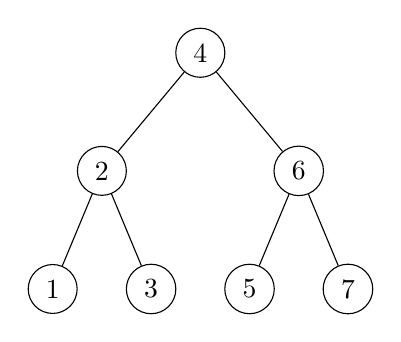
\begin{tikzpicture}[
  every node/.style = {minimum width = 1em, draw, circle},
  level/.style = {sibling distance = 25mm/#1}
  ]
  \node {4}
  child {node {2} 
        child {node {1}}
        child {node {3}}
        }
  child {node {6}
        child {node {5}}
        child {node {7}}
        };
\end{tikzpicture}
            \caption{Best case: 
            Adding nodes in \emph{pre-order} gives the tree a well-balanced shape.
            Level-by-level order works as well}
            \label{fig:wellbalanced}
        \end{subfigure}
        % \hfill
        \begin{subfigure}[h]{0.45\textwidth}
            \centering
\begin{tikzpicture}[
  every node/.style = {minimum width = 2em, draw, circle},
  level/.style = {sibling distance = 30mm/#1}
  ]
  \node {1}
  child {edge from parent}
  child {node {2} 
        child {edge from parent}
        child {node {3}
               child {edge from parent}
               child {node {4}
                    child {edge from parent}
                    child {node {5}
                        child {edge from parent}
                        child {node {6}
                            child {edge from parent}
                            child {node {7}}
                        }
                    }
               }
        }
  };
\end{tikzpicture}
            \caption{Worst case:
            Adding nodes \emph{in-order}, gives the tree a shape of a singly
            linked list}
            \label{fig:unbalanced}
        \end{subfigure}
        \caption{Why shape and order matters}
        \label{bstshape}
    \end{figure}
    At worst, a basic BST operation like \hyperref[sec:adding]{adding, updating} 
    and \hyperref[sec:lookup]{\mintinline{julia}{lookup}}, locates a node $n$ in a tree
    of height $h$ in $O(h)$ time. 
    A ''well-balanced'' binary tree will have a height of $(\log n)$, 
    giving basic operations a time complexity of $O(\log n)$.
    Adding nodes with keys in increasing (or decreasing) order 
    defeats this logarithmic performance. Requiring instead a 
    time-cost proportional to the length of the tree. The length being the
    number of nodes in the tree. 
    For example one should add seven nodes either in 
    pre-order (4, 2, 1, 3, 6, 5, 7) or
    level-by-level (4, 2, 6, 1, 3, 5, 7) as in \autoref{fig:wellbalanced}
    rather than inorder (1, 2, 3, 4, 5, 6, 7) as in \autoref{fig:unbalanced}.
    One can expect that a tree that was built on a random set of keys $n$,
    like in the case of our benchmark, 
    will roughly get a height of $\log n$. As one can clearly see in the benchmark 
    result in \autoref{fig:fig1} and \autoref{tab:growth}.
\end{document}